% lint-skip: 未完成ステータス（figure/table caption 未対応，人手チェック時に解消予定）
\documentclass[../../main.tex]{subfiles}
\begin{document}

\begin{flushright}
  \footnotesize\textit{【自動文字起こし・要確認】}
\end{flushright}

[解] 時刻 $t$ での水面の面積 $P$ とすると，
\[ -S v = P \dfrac{dx}{dt} \quad \cdots \text{①} \]
ここで，
\[ P = \pi \left( \dfrac{x}{h} R \right)^2 = \dfrac{\pi R^2}{h^2} x^2 \quad \cdots \text{②} \]
及び
\[ v = k x \]
を①に代入して
\[ -S k x = \dfrac{\pi R^2}{h^2} x^2 \dfrac{dx}{dt} \]
$x > 0$ より，
\[ -S k = \dfrac{\pi R^2}{h^2} x \dfrac{dx}{dt} \]
両辺積分して，$t = 0$ で $x = h$ より，
\[ -S k t + \dfrac{1}{2} \pi R^2 = \dfrac{1}{2} \dfrac{\pi R^2}{h^2} x^2 \]
$x > 0$ より，
\[ x(t) = \sqrt{\dfrac{2h^2}{\pi R^2} \left( \dfrac{1}{2} \pi R^2 - Skt \right)} \]

\begin{figure}[htb]
  \centering
  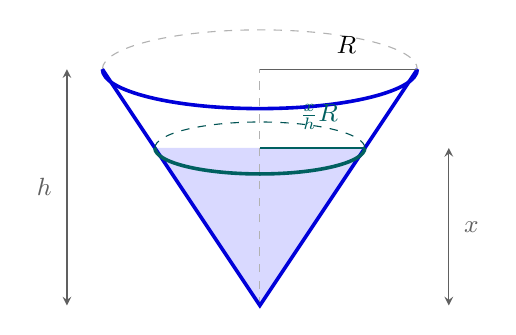
\begin{tikzpicture}[>=stealth,
    every node/.style={font=\small}]
    % The example shows x/h=2/3, hence the water radius is 2R/3.
    \fill[blue!15] (-1.333,-1) -- (0,-3) -- (1.333,-1) -- cycle;
    \draw[dashed, gray!60] (0,-3) -- (0,0);
    \draw[dashed, gray!60]
    (-2,0) arc (180:0:2cm and 0.5cm);
    \draw[line width=1.3pt, blue!85!black]
    (-2,0) -- (0,-3) -- (2,0);
    \draw[line width=1.3pt, blue!85!black]
    (-2,0) arc (180:360:2cm and 0.5cm);
    \draw[dashed, teal!65!black]
    (-1.333,-1) arc (180:0:1.333cm and 0.33cm);
    \draw[line width=1.3pt, teal!75!black]
    (-1.333,-1) arc (180:360:1.333cm and 0.33cm);
    \draw[<->, gray!75!black] (-2.45,-3) -- (-2.45,0)
    node[midway,left=2pt] {$h$};
    \draw[<->, gray!75!black] (2.4,-3) -- (2.4,-1)
    node[midway,right=2pt] {$x$};
    \draw[gray!75!black] (0,0) -- (2,0);
    \draw[teal!75!black] (0,-1) -- (1.333,-1);
    \node[above=2pt] at (1.1,0) {$R$};
    \node[above=3pt, teal!75!black] at (0.75,-1)
    {$\frac{x}{h}R$};
  \end{tikzpicture}
  \caption{円錐容器の水位 $x$ と水面の半径 $Rx/h$}
\end{figure}

\end{document}
